\documentclass[12pt, letterpaper]{article}
\usepackage{lmodern}
\usepackage[T1]{fontenc}
\usepackage{amsmath}
\usepackage{float}
\usepackage{amsthm}
\usepackage{esvect}
\usepackage[toc,page]{appendix}
\usepackage{leftidx}
\usepackage{color}
\usepackage{framed, color}
\usepackage{multirow}
\usepackage{pdfpages}
\usepackage{multicol}
\usepackage{wrapfig,lipsum,booktabs}
\usepackage[utf8]{inputenc}
\usepackage{mathtools,hyperref}
\hypersetup{
    colorlinks=true,
    linkcolor=cyan,
    filecolor=cyan,      
    urlcolor=red,
    citecolor=red,
}
\usepackage{cleveref}
\usepackage{commath}
\usepackage{enumitem}
\usepackage{amssymb}
\renewcommand{\qedsymbol}{$\blacksquare$}
%%%%%%%%%%%
%%%%%%%%%%%  User Defined Commands. (macros)
%%%%%%%%%%%

\definecolor{mgreen}{RGB}{25,147,100}
\definecolor{shadecolor}{rgb}{1,.8,.1}
\definecolor{shadecolor2}{RGB}{245,237,0}
\definecolor{orange}{RGB}{255,137,20}
\definecolor{orange}{RGB}{245,37,100}

\usepackage{graphicx}
\usepackage{subcaption}


%%%%%%%
%%%%%%%%%%%
%%%%%%%%%%%%%%%%%%
%%%%%%%%%%%%%%%%%%%%%%%%%%%%
\usepackage[english]{babel}
\usepackage[utf8]{inputenc}
\usepackage{fancyhdr}

\pagestyle{fancy}

%%%%%%%%%%%%%%%%%%%%%%%%%%%%%%%%%%%%%%%%%%%%%%%%%%

\fancyhf{}
\rhead{}
%\lhead{Help}
\renewcommand{\headrulewidth}{0pt}
%\futurelet\TMPfootrule\def\headrule{{\color{Cerulean}\TMPfootrule}}



\lfoot{Page \thepage}
%\rfoot{hnoorazar.com, h.noorazar@gmail.com}
\renewcommand{\footrulewidth}{2pt}
\futurelet\TMPfootrule\def\footrule{{\color{Cerulean}\TMPfootrule}}

%%
%%%%%%%%%%%%%%%%%%%%%%%%%%%%

%\usepackage[utf8]{inputenc}
% \usepackage{tgbonum}
%%%%%%%%%%%%%%%%%%%%%%%%%%%%
%%%%%%%%%%%%%%%%%%%%%%%%%%%% color horizontal line
%%%%%%%%%%%%%%%%%%%%%%%%%%%%

\usepackage[x11names, dvipsnames]{xcolor}
\usepackage{lipsum}
\usepackage[textwidth = 15cm]{geometry}

\newlength{\seplinewidth}
\newlength{\seplinesep}
\setlength{\seplinewidth}{1mm}
\setlength{\seplinesep}{2mm}
\colorlet{sepline}{PaleVioletRed3}
\newcommand*{\sepline}{%
  \par
  \vspace{\dimexpr\seplinesep+.5\parskip}%
  \cleaders\vbox{%
    \begingroup % because of color
      \color{sepline}%
      \hrule width\linewidth height\seplinewidth
    \endgroup
  }\vskip\seplinewidth
  \vspace{\dimexpr\seplinesep-.5\parskip}%
}
%%%%%%%%%%%%%%%%%%%%%%%%%%%
%%%%%%%%%%%%%%%%%%%%%%%%%%%
%%%%%%%%%%%%%%%%%%%%%%%%%%%
\def\code#1{\textbf{\texttt{#1}}}
\def\vari#1{{\color{Cerulean}{\textbf{\texttt{#1}}}}}
\def\func#1{{\color{Maroon}{\textbf{\texttt{#1}}}}}
\newenvironment{coded}{\color{blue}\code}
%%%%%%%%%%%%%%%%%%%%%%%%%%%
%%%%%%%%%%%%%%%%%%%%%%%%%%%


\begin{document}
\date{}
\title{To scale or not, before PCA}
\maketitle
\vspace{-.88in}
\sepline


PCA represents the data in a new coordinate system
 so the first direction/dimension has the maximum variance, 
 with maximum information. 

If one variable, $v_1$ , is in a scale 
that varies from -10M to 10M, like 
distance between cities in meters,
and another, $v_2$, from -1 to 1, then just 
due to scale difference, variance of $v_1$ 
would be larger, and picked by PCA process.

Hence, one should do the standardization before applying PCA. 

(standardization keeps correlations fixed, mix-max scaling changes it.)

Let's take a look:


\begin{figure}[h]
    \centering
    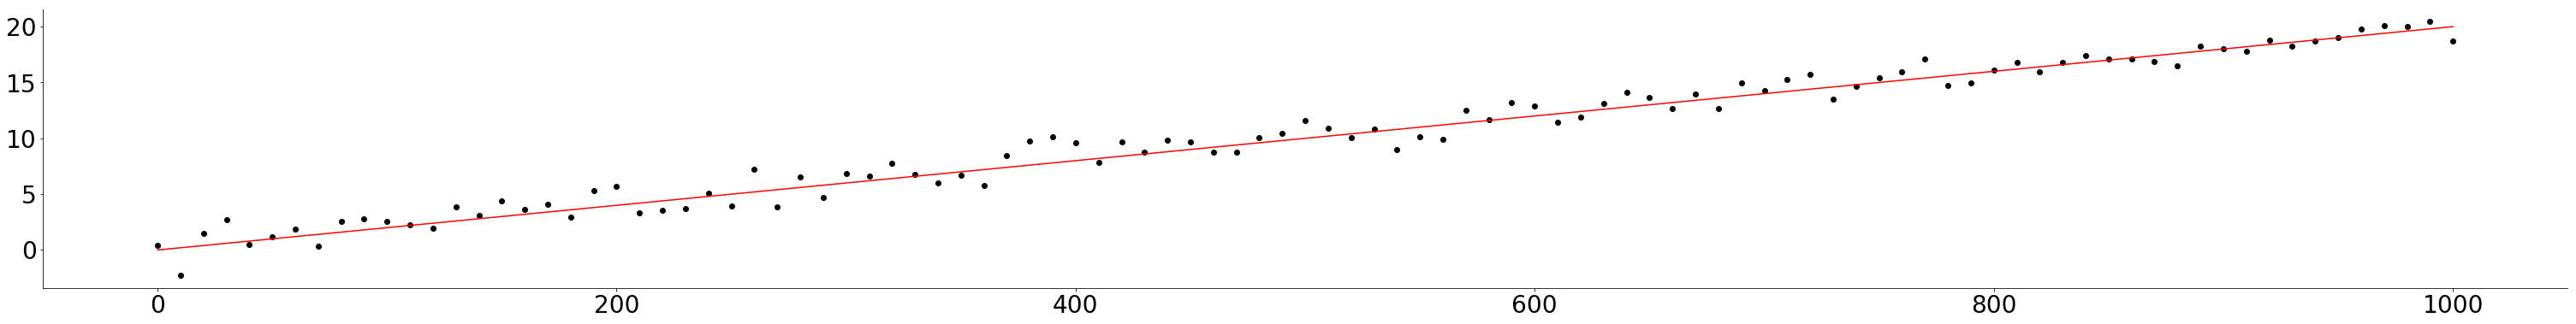
\includegraphics[width=1\textwidth]{1.png}
    \caption{}
    \label{fig:areaPrice}
\end{figure}

In Fig.~\ref{fig:areaPrice}, the range in the $x$-direction is 1000 
and in the $y$-direction is 20, so, variance 
in $x$-direction will be larger as well. Hence we normalize. (Fig.~\ref{fig:areaPrice2})

\begin{figure}[H]
    \centering
    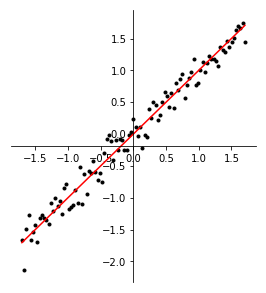
\includegraphics[width=.4\textwidth]{2.png}
    \caption{}
    \label{fig:areaPrice2}
\end{figure}

Now the data are in almost the same range, 
we rotate the coordinate system so first 
axis is in the direction of the derived variable 
with largest variance and second will be 
in the direction of second largest orthogonal to previous one.

In the above plot the red line would be 
the first PCA, let me call it $PC_1$ 
direction and a line orthogonal to it will be the second direction, $PC_2$. 

However, even after mapping
the data to PCA space (Fig.~\ref{fig:areaPrice3}), 
in the new coordinate system you can see, the new variables will be in different scales. The data in direction of the $PC_1$ has larger variance as opposed to the $PC_2$. 

Hence, if we want to compute distances 
in the PCA space, the distances will be 
affected by such a difference in scale. 
So, we have to do another scaling, after the PCA step.

In conclusion
\begin{itemize}
   \item The scaling done in the first step lets PCA does its job correctly.
   \item  The scaling in the last step makes the computed distances to not be affected by difference of scales
\end{itemize}
Representing the data
in PCA space kills the correlation among 
variables, hence the covariance in PCA space is diagonal:


\begin{figure}[h]
    \centering
    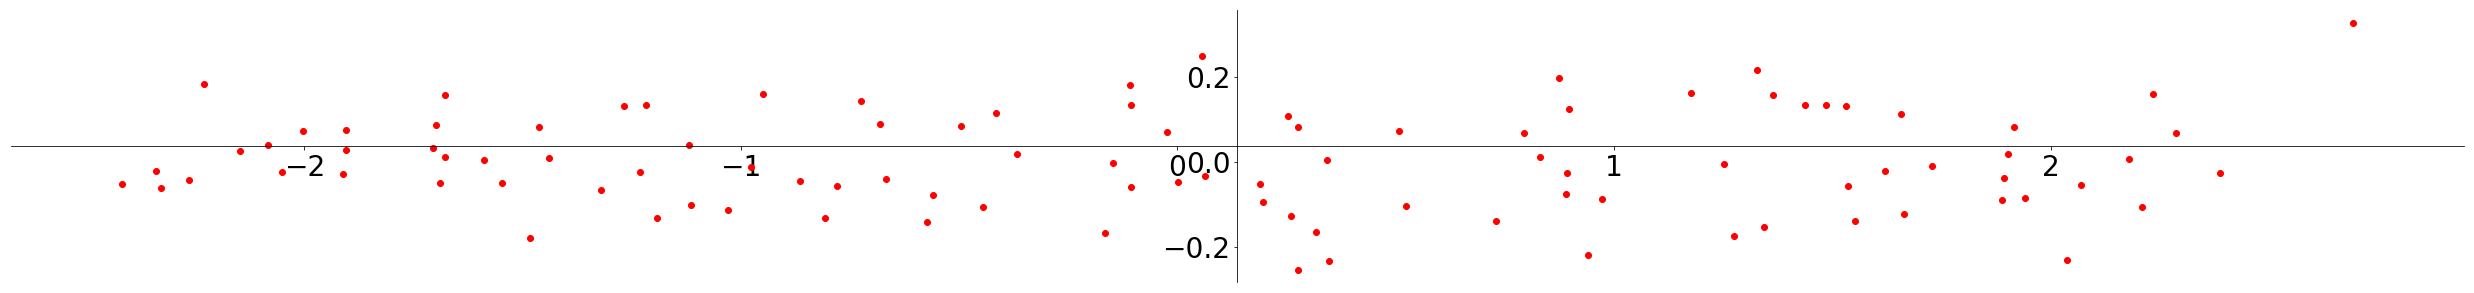
\includegraphics[width=1\textwidth]{3.png}
    \caption{}
    \label{fig:areaPrice3}
\end{figure}



And the second scaling kills the bad effect of different scales in computing distances. 

The three sptes described above, scaling, PCA step, scaling, is equivalent to \emph{Mahalanobis} distance.
It kills the effect of scales and correlations among data.

To see the proof of the equivalency please take a look
\href{https://static1.squarespace.com/static/5a4c161cfe54ef45b17aa18e/t/5cbc0736ecaa100001bf4240/1555826488060/mahab_equal.pdf}{here}.


\end{document}
